\section{Writing}
\paragraph{Part A}
\subparagraph{51.Directions:}

Write an e-mail of about 100 words to a foreign teacher in your college, inviting him/her to be a judge for the upcoming English speech contest.

You should include the details you think necessary.

You should write neatly on the ANSWER SHEET.

Do not sign your own name at the end of the e-mail. Use ``Li Ming'' instead.

Do not write the address. (10 points)

\paragraph{Part B}
\subparagraph{52.Directions:}

Write an essay of 160-200 words based on the following drawing .In your essay, you should

1) describe the drawing briefly.

2) interpret its intended meaning ,and

3) give your comments.

You should write neatly on the ANSWER SHEET 2. (20points)

\begin{center}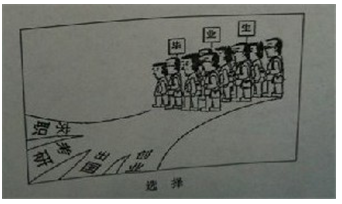
\includegraphics[width=14cm]{8.png}\end{center}